\documentclass{standalone}
\usepackage{fkmath}
\usepackage{tikz}
\begin{document}
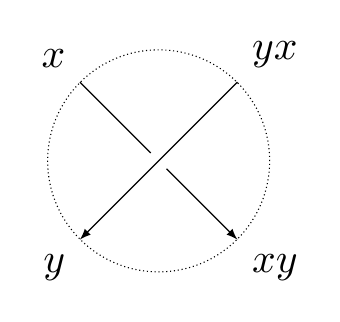
\begin{tikzpicture}[every node/.style={scale=1.5}]
  \draw[-latex] (-1,1) -- (1,-1) node[at start, above left] {$x$} node[at end, below right] {$x \underop y$};
  \draw[white, line width=8pt] (1,1) -- (-1,-1);
  \draw[-latex] (1,1) -- (-1,-1) node[at start, above right] {$y \overop x$} node[at end, below left] {$y$};
  \draw[densely dotted] (0,0) circle (1.41);
\end{tikzpicture}
\end{document}
